\documentclass[border=10pt,12pt]{standalone}
\usepackage[scaled]{helvet}
\usepackage[T1]{fontenc}
\renewcommand\familydefault{\sfdefault}

\usepackage{tikz}
\usetikzlibrary{arrows.meta, positioning, calc}

\definecolor{knowFill}{HTML}{EAF1F7}
\definecolor{knowLine}{HTML}{315C86}
\definecolor{divFill}{HTML}{E6EBD2}
\definecolor{divLine}{HTML}{6F7F3D}
\definecolor{belongFill}{HTML}{F7F4EC}
\definecolor{belongLine}{HTML}{333333}
\definecolor{stone}{HTML}{EFE9DD}
\definecolor{warn}{HTML}{B3261E}

% Draw one classical column: #1 = centre x, #2 = shaft fill, #3 = structural line
\newcommand{\drawcolumn}[3]{%
  \fill[#3] ({#1-1.65},0.55) rectangle ({#1+1.65},1.20);                       % base
  \fill[#2,draw=#3,line width=1pt] ({#1-1.40},1.20) rectangle ({#1+1.40},8.40);% shaft
  \foreach \fx in {-0.90,-0.30,0.30,0.90}{%
    \pgfmathsetmacro\px{#1+(\fx)}%
    \draw[#3!35,line width=0.5pt] (\px,1.45) -- (\px,8.2);%
  }
  \fill[#3] ({#1-1.65},8.40) rectangle ({#1+1.65},9.45);                       % capital
  \draw[#3,line width=1pt] ({#1-1.86},9.45) rectangle ({#1+1.86},9.80);        % abacus
}

\begin{document}

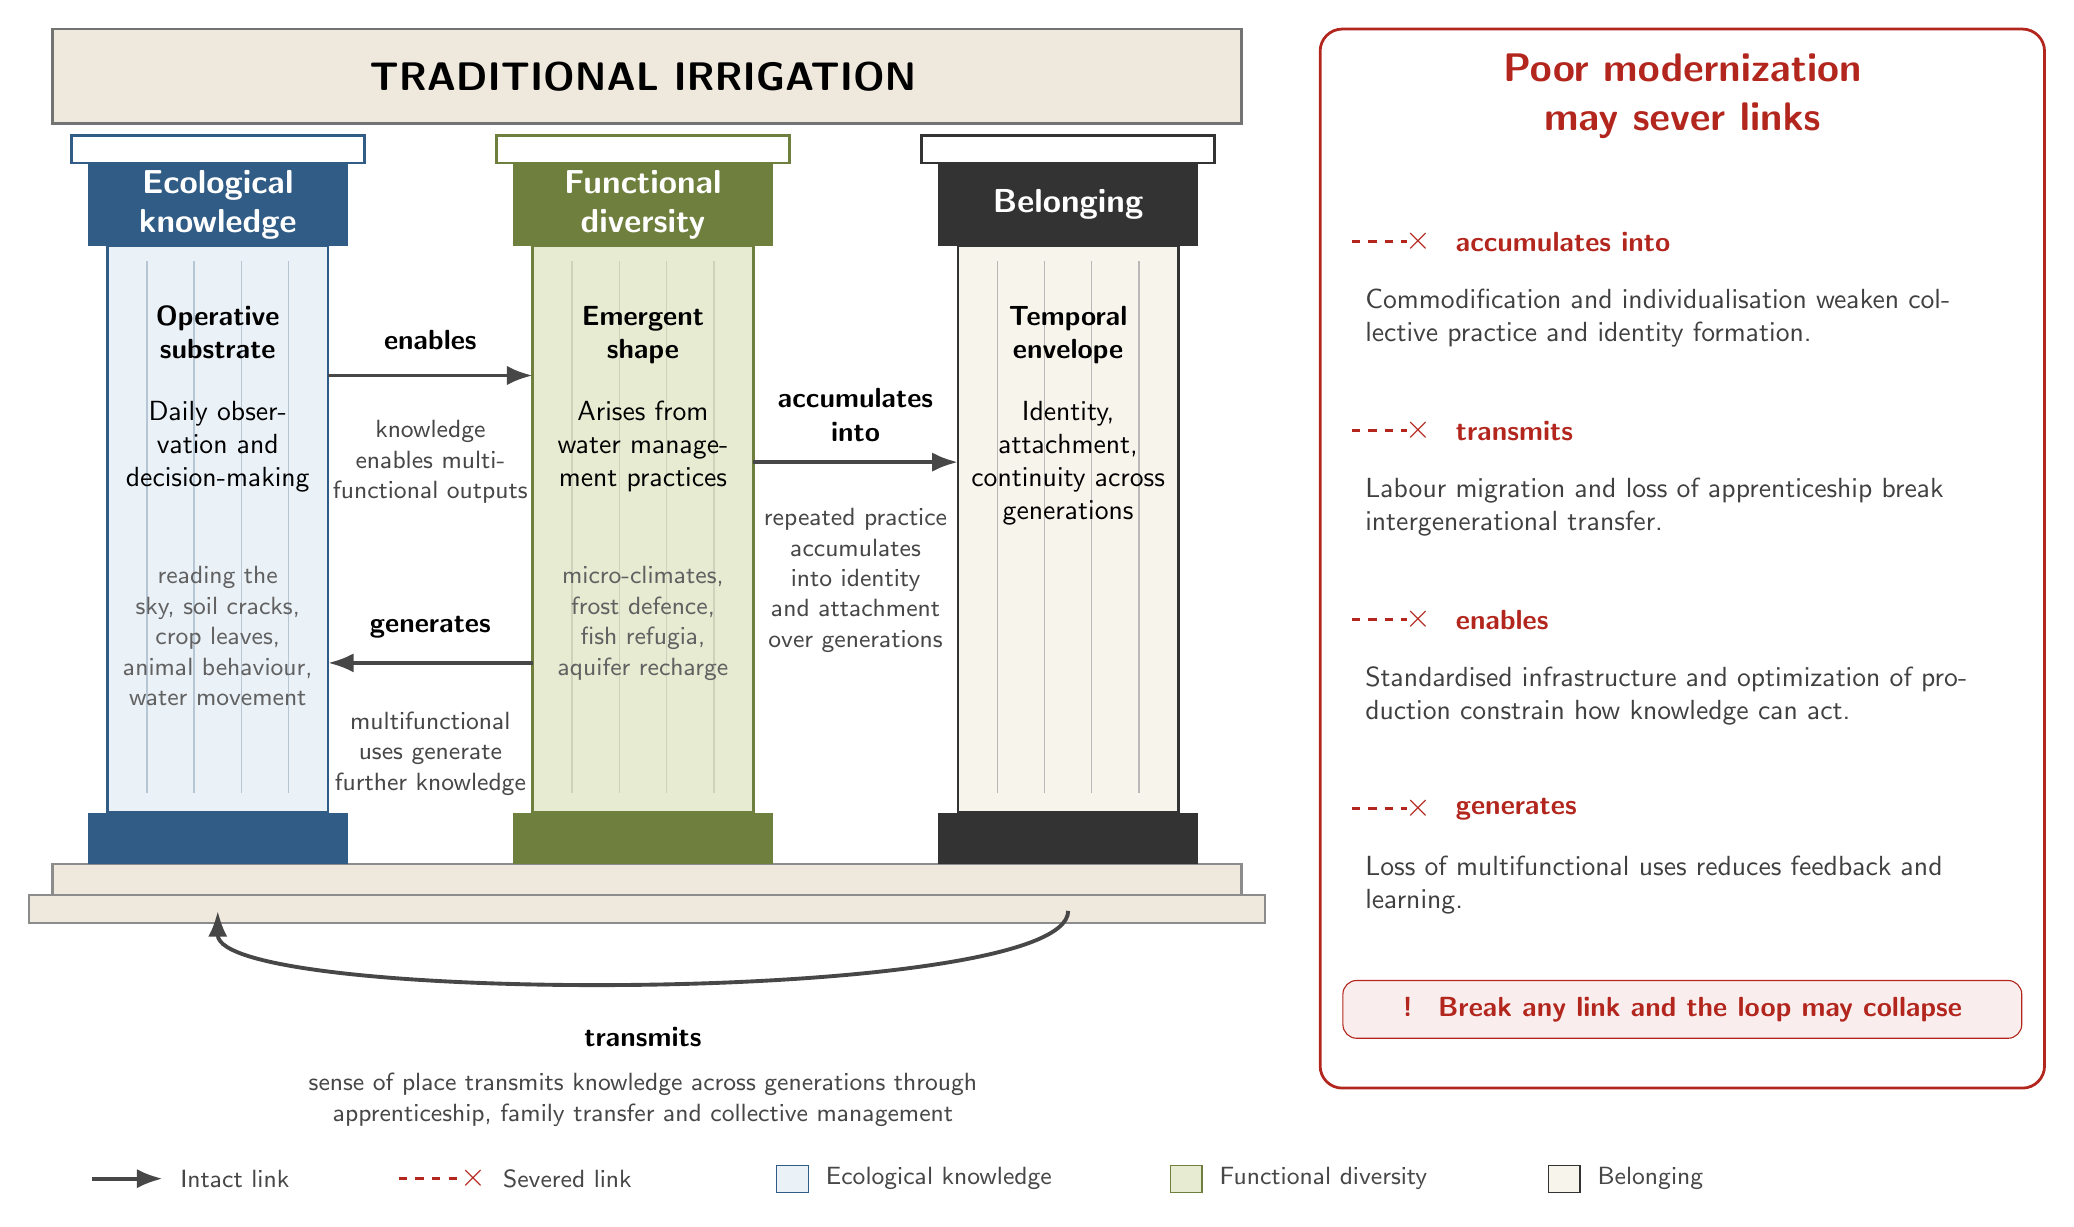
\begin{tikzpicture}[
  font=\sffamily,
  >=Latex,
  capname/.style  ={font=\large\bfseries, text=white, align=center},
  subtitle/.style ={font=\normalsize\bfseries, align=center},
  body/.style     ={font=\normalsize, align=center},
  egs/.style      ={font=\small, align=center, text=black!62},
  flow/.style     ={->, line width=1.4pt, draw=black!72},
  flowlab/.style  ={font=\normalsize\bfseries, align=center},
  note/.style     ={font=\small, align=center, text=black!72},
  sever/.style    ={warn, dashed, line width=1.3pt},
  xmark/.style    ={warn, font=\bfseries\large},
  modlink/.style  ={font=\normalsize\bfseries, text=warn, anchor=west},
  modnote/.style  ={font=\normalsize, align=left, text=black!75, anchor=north west}
]

% =========================================================
% STYLOBATE + ENTABLATURE (the system the pillars hold up)
% =========================================================

\fill[stone,draw=black!45,line width=0.8pt] (0.2,-0.20) rectangle (15.9,0.15);
\fill[stone,draw=black!45,line width=0.8pt] (0.5,0.15) rectangle (15.6,0.55);

\fill[stone,draw=black!55,line width=1pt] (0.5,9.95) rectangle (15.6,11.15);
\node[font=\Large\bfseries] at (8.0,10.55) {TRADITIONAL IRRIGATION};

% =========================================================
% THREE PILLARS
% =========================================================

\drawcolumn{2.6}{knowFill}{knowLine}
\drawcolumn{8.0}{divFill}{divLine}
\drawcolumn{13.4}{belongFill}{belongLine}

% Names on the capitals (white) ---------------------------
\node[capname, text width=3.05cm] at (2.6,8.92)  {Ecological knowledge};
\node[capname, text width=3.05cm] at (8.0,8.92)  {Functional diversity};
\node[capname, text width=3.05cm] at (13.4,8.92) {Belonging};

% Ecological knowledge ------------------------------------
\node[subtitle, anchor=north, text width=2.55cm] at (2.6,7.75) {Operative substrate};
\node[body,     anchor=north, text width=2.55cm] at (2.6,6.55) {Daily observation and decision-making};
\node[egs,      anchor=north, text width=2.55cm] at (2.6,4.45)
  {reading the sky, soil cracks, crop leaves, animal behaviour, water movement};

% Functional diversity ------------------------------------
\node[subtitle, anchor=north, text width=2.55cm] at (8.0,7.75) {Emergent shape};
\node[body,     anchor=north, text width=2.55cm] at (8.0,6.55) {Arises from water management practices};
\node[egs,      anchor=north, text width=2.55cm] at (8.0,4.45)
  {micro-climates, frost defence, fish refugia, aquifer recharge};

% Belonging -----------------------------------------------
\node[subtitle, anchor=north, text width=2.55cm] at (13.4,7.75) {Temporal envelope};
\node[body,     anchor=north, text width=2.55cm] at (13.4,6.55) {Identity, attachment, continuity across generations};

% =========================================================
% REINFORCING FLOWS BETWEEN PILLARS
% =========================================================

% knowledge -> diversity : enables (upper)
\draw[flow] (4.0,6.75) -- (6.6,6.75);
\node[flowlab] at (5.3,7.20) {enables};
\node[note, text width=2.55cm] at (5.3,5.65)
  {knowledge enables multifunctional outputs};

% diversity -> knowledge : generates (lower)
\draw[flow] (6.6,3.10) -- (4.0,3.10);
\node[flowlab] at (5.3,3.55) {generates};
\node[note, text width=2.55cm] at (5.3,1.95)
  {multifunctional uses generate further knowledge};

% diversity -> belonging : accumulates into
\draw[flow] (9.4,5.65) -- (12.0,5.65);
\node[flowlab, text width=2.6cm] at (10.7,6.25) {accumulates into};
\node[note, text width=2.55cm] at (10.7,4.15)
  {repeated practice accumulates into identity and attachment over generations};

% belonging -> knowledge : transmits (shallow arc through the foundation)
\draw[flow] (13.4,-0.05) .. controls (13.4,-1.25) and (2.6,-1.25) .. (2.6,-0.05);
\node[flowlab] at (8.0,-1.65) {transmits};
\node[note, text width=13cm] at (8.0,-2.45)
  {sense of place transmits knowledge across generations through apprenticeship,
   family transfer and collective management};

% =========================================================
% MODERNISATION PANEL (right)
% =========================================================

\draw[warn, line width=1pt, rounded corners=8pt] (16.6,-2.30) rectangle (25.8,11.15);

\node[font=\Large\bfseries, text=warn, align=center, text width=8.8cm]
  at (21.2,10.30) {Poor modernization\\may sever links};

% one severed link per reinforcing flow
\foreach \y/\lab/\txt in {%
  8.45/{accumulates into}/{Commodification and individualisation weaken collective
        practice and identity formation.},
  6.05/{transmits}/{Labour migration and loss of apprenticeship break
        intergenerational transfer.},
  3.65/{enables}/{Standardised infrastructure and optimization of production
        constrain how knowledge can act.},
  1.25/{generates}/{Loss of multifunctional uses reduces feedback and learning.}%
}{%
  \draw[sever] (17.0,\y) -- (17.7,\y);
  \node[xmark] at (17.85,\y) {$\times$};
  \node[modlink] at (18.2,\y) {\lab};
  \node[modnote, text width=7.7cm] at (17.05,{\y-0.48}) {\txt};
}

\node[draw=warn, fill=warn!8, rounded corners=5pt, font=\normalsize\bfseries,
      text=warn, align=center, text width=8.2cm, inner sep=6pt]
  at (21.2,-1.30) {! \ Break any link and the loop may collapse};

% =========================================================
% LEGEND
% =========================================================

\draw[flow] (1.0,-3.45) -- (1.9,-3.45);
\node[note, anchor=west] at (2.0,-3.45) {Intact link};

\draw[sever] (4.9,-3.45) -- (5.7,-3.45);
\node[xmark] at (5.85,-3.45) {$\times$};
\node[note, anchor=west] at (6.1,-3.45) {Severed link};

\fill[knowFill,draw=knowLine] (9.7,-3.62) rectangle (10.1,-3.28);
\node[note, anchor=west] at (10.2,-3.45) {Ecological knowledge};

\fill[divFill,draw=divLine] (14.7,-3.62) rectangle (15.1,-3.28);
\node[note, anchor=west] at (15.2,-3.45) {Functional diversity};

\fill[belongFill,draw=belongLine] (19.5,-3.62) rectangle (19.9,-3.28);
\node[note, anchor=west] at (20.0,-3.45) {Belonging};

\end{tikzpicture}

\end{document}
